\subsection*{Kroswalidacja zwykła}

\begin{figure}[H]
    \center
    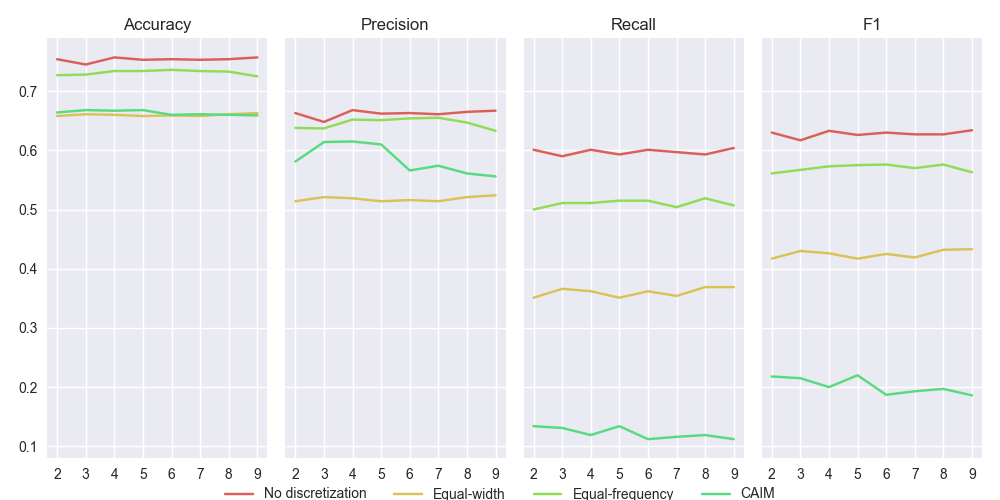
\includegraphics[width=0.9\textwidth]{img/cv_scores_kfold/scoring_kfold_diabetes.png}
    \caption{Wartości metryk dla klasyfikatora Bayesowskiego.}
\end{figure}

\begin{figure}[H]
    \center
    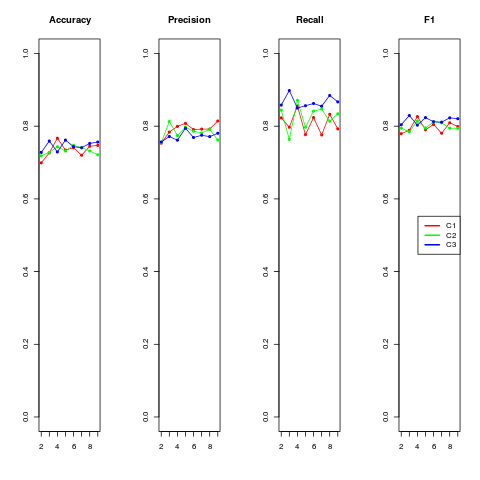
\includegraphics[width=0.9\textwidth]{img/cv_plots/cv_ns_diabetes.png}
    \caption{Wartości metryk dla drzewa decyzyjnego C4.5.}
\end{figure}

\begin{table}[H]
  \center
\begin{tabular}{|c|c|c|c|c|c|c|c|c|c|}  \hline
  \multicolumn{2}{|c|}{} & \multicolumn{8}{c|}{Liczba foldów} \\ \hline
Konfiguracja &    Metryka &     2 &     3 &     4 &     5 &     6 &     7 &     8 &     9 \\ \hline
          C1 &   Accuracy &  0.70 &  0.73 &  0.77 &  0.73 &  0.74 &  0.72 &  0.74 &  0.75 \\ \hline
          C1 &  Precision &  0.75 &  0.78 &  0.80 &  0.81 &  0.79 &  0.79 &  0.79 &  0.81 \\ \hline
          C1 &     Recall &  0.82 &  0.80 &  0.86 &  0.78 &  0.82 &  0.78 &  0.83 &  0.79 \\ \hline
          C1 &         F1 &  0.78 &  0.79 &  0.83 &  0.79 &  0.80 &  0.78 &  0.81 &  0.80 \\ \hline \hline
          C2 &   Accuracy &  0.72 &  0.73 &  0.74 &  0.73 &  0.75 &  0.74 &  0.73 &  0.72 \\ \hline
          C2 &  Precision &  0.75 &  0.81 &  0.77 &  0.80 &  0.79 &  0.78 &  0.79 &  0.76 \\ \hline
          C2 &     Recall &  0.84 &  0.76 &  0.87 &  0.80 &  0.84 &  0.85 &  0.81 &  0.83 \\ \hline
          C2 &         F1 &  0.79 &  0.78 &  0.81 &  0.80 &  0.81 &  0.81 &  0.79 &  0.79 \\ \hline \hline
          C3 &   Accuracy &  0.73 &  0.76 &  0.73 &  0.76 &  0.74 &  0.74 &  0.75 &  0.76 \\ \hline
          C3 &  Precision &  0.76 &  0.77 &  0.76 &  0.79 &  0.77 &  0.78 &  0.77 &  0.78 \\ \hline
          C3 &     Recall &  0.86 &  0.90 &  0.85 &  0.86 &  0.86 &  0.86 &  0.88 &  0.87 \\ \hline
          C3 &         F1 &  0.80 &  0.83 &  0.80 &  0.82 &  0.81 &  0.81 &  0.82 &  0.82 \\ \hline
\end{tabular}
  \caption{Dokładne wartości metryk dla drzewa decyzyjnego C4.5.}
\end{table}
